\documentclass[conference]{IEEEtran}
\IEEEoverridecommandlockouts
% The preceding line is only needed to identify funding in the first footnote. If that is unneeded, please comment it out.
\usepackage{cite}
\usepackage{amsmath,amssymb,amsfonts}
\usepackage{algorithmic}
\usepackage{graphicx}
\usepackage{textcomp}
\usepackage{xcolor}
\usepackage{float}
\usepackage[utf8]{inputenc}
\usepackage[T5]{fontenc}
\usepackage[vietnamese,english]{babel}
\usepackage{tikz}
\usepackage[table]{xcolor}


\pagestyle{plain}



\usetikzlibrary{arrows.meta, positioning}

\def\BibTeX{{\rm B\kern-.05em{\sc i\kern-.025em b}\kern-.08em
    T\kern-.1667em\lower.7ex\hbox{E}\kern-.125emX}}
    \makeatletter
\newcommand{\linebreakand}{%
  \end{@IEEEauthorhalign}
  \hfill\mbox{}\par
  \mbox{}\hfill\begin{@IEEEauthorhalign}
}
\makeatother
\begin{document}


\title{
    Enhancing Speech Extraction And Speaker Recognition Through Machine Learning And Deep Learning Integration\\
}

\author{
    \IEEEauthorblockN{1\textsuperscript{st} Cao Hoài Sang}
    \IEEEauthorblockA{\textit{Department of Information Systems} \\
        \textit{University of Information Technology} \\
        Ho Chi Minh City, Viet Nam \\
        21522541@gm.uit.edu.vn}
    %
    \and
    %
    \IEEEauthorblockN{2\textsuperscript{nd} Thi Thành Công}
    \IEEEauthorblockA{\textit{Department of Information Systems} \\
        \textit{University of Information Technology} \\
        Ho Chi Minh City, Viet Nam \\
        21521897@gm.uit.edu.vn}
        %
        \linebreakand
        \IEEEauthorblockN{3\textsuperscript{th} Nguyễn Minh Nhựt}
        \IEEEauthorblockA{\textit{Department of Information Systems} \\
        \textit{University of Information Technology} \\
        Ho Chi Minh City, Viet Nam \\
        nhutnm.17@grad.uit.edu.vn}
    %
    \and
    \IEEEauthorblockN{4\textsuperscript{rd} Nguyễn Đình Thuân}
    \IEEEauthorblockA{\textit{Department of Information Systems} \\
        \textit{University of Information Technology} \\
        Ho Chi Minh City, Viet Nam \\
        thuannd@uit.edu.vn}
}

\maketitle

\begin{abstract}
    In the age of digital communication and telework, the need for advanced conversation processing becomes increasingly important.
    This study proposes a system capable of speech separation and speaker recognition.
    The approach combines acoustic features such as MFCC, XVector, DVector and Wavelet with machine learning including HMM or deep learning models like
    RNN and QCNN. The system is trained and tested on a labeled conversation dataset.
    Experimental results demonstrate that the system achieves high accuracy in speaker discrimination and speech extraction.
\end{abstract}


\section{Introduction}

With the increasing prevalence of online meetings, virtual collaboration, and remote communication, the demand for accurate and real-time speech processing systems has become more urgent than ever. Traditional automatic speech recognition (ASR) systems primarily focus on transcribing spoken content into text. However, these systems often fall short in distinguishing between different speakers and in isolating clean speech signals from overlapping conversations or background noise.

This research addresses these limitations by proposing an integrated framework that enhances both speech extraction and speaker recognition. By leveraging a combination of acoustic feature representations—such as MFCC, Wavelet, X-Vector, and D-Vector—and advanced modeling techniques including Hidden Markov Models (HMM), Recurrent Neural Networks (RNN), and Quantum Convolutional Neural Networks (QCNN), our approach aims to significantly improve the performance and robustness of ASR systems in real-time multi-speaker environments.

The proposed method is especially relevant for applications requiring speaker-aware transcription, speaker diarization, and secure voice-based authentication, where both accuracy and adaptability are critical.

\section{Related Work}

In the field of speech recognition and analysis, multiple approaches have been proposed with the aid of machine learning and deep learning techniques. This section presents an overview of the relevant approaches, divided into groups based on the characteristic methodology and the model used.

\subsection{Mel-Frequency Cepstral Coefficients (MFCC)}

MFCC is one of the most common features in speech signal processing. The article on the use of MFCC to extract characteristics for training HMM models (hidden Markov models) by Rabiner~\cite{rabiner1989tutorial} detailed the use of hidden Markov models (HMM) combined with MFCC characteristics for speech recognition.

\subsection{Wavelet-based Features}

Wavelet transform is a powerful tool used to exploit time and frequency information from audio signals. Wavelet shows good ability to handle sound in noisy or unstable environments. Although not as widely used as MFCC, wavelets have recently been applied to systems thanks to their powerful noise cancellation capabilities. Studies have shown that using wavelet transforms in feature extraction can improve the accuracy of speech recognition systems, particularly in environments with noise~\cite{gupta2003robust, wang2008robust}.

\subsection{X-vector and D-vector Embeddings}

X-vectors and D-vectors are representations learned from audio data, often used for speaker recognition. X-vector systems typically employ DNN or TDNN networks to learn embeddings that improve speaker discrimination accuracy. These representations are widely used in modern processing pipelines, such as those in Kaldi and SpeechBrain. Snyder et al.~\cite{Snyder2018Xvectors} introduced X-vector as a deep learning representation for speaker recognition. For D-vector, Wan et al.~\cite{Wan2018Generalized} proposed using the GE2E loss function for training, which improves performance in speaker recognition.

\subsection{Hidden Markov Models (HMM)}

HMM forms the foundation of many traditional ASR systems. Rabiner~\cite{rabiner1989tutorial} proposed effective Viterbi training methods and algorithms for HMM in speech recognition. Hybrid systems, as discussed in~\cite{voll2007hybrid, perero2022comparison}, have shown that combining HMM with neural networks can enhance accuracy in diverse environments.

\subsection{Recurrent Neural Networks (RNN)}

RNNs are widely used in ASR tasks because they can capture temporal dependencies in speech data. LSTM and GRU variants effectively address vanishing gradient problems and model long-term context. Systems like Deep Speech~\cite{hannun2014deep} and the work of Graves et al.~\cite{graves2013speech} show that RNN-based models can achieve good results in end-to-end ASR tasks

\subsection{Quantum Convolutional Neural Networks (QCNN)}

QCNN is a novel model in quantum deep learning, designed to leverage quantum properties to reduce redundant parameters, focus on key features, and enhance representability. Cong et al.~\cite{Cong2019QuantumCNN} introduced QCNN as a new quantum machine learning model that combines features of convolutional neural networks with quantum mechanisms to classify quantum states. Although QCNN has not yet been widely applied in ASR, research by Yang et al.~\cite{Yang2021Decentralizing} shows its potential when combined with classical methods.

\section{Background}


\begin{figure}[H]
    \centering
    \begin{minipage}{0.5\textwidth}
        \centering
        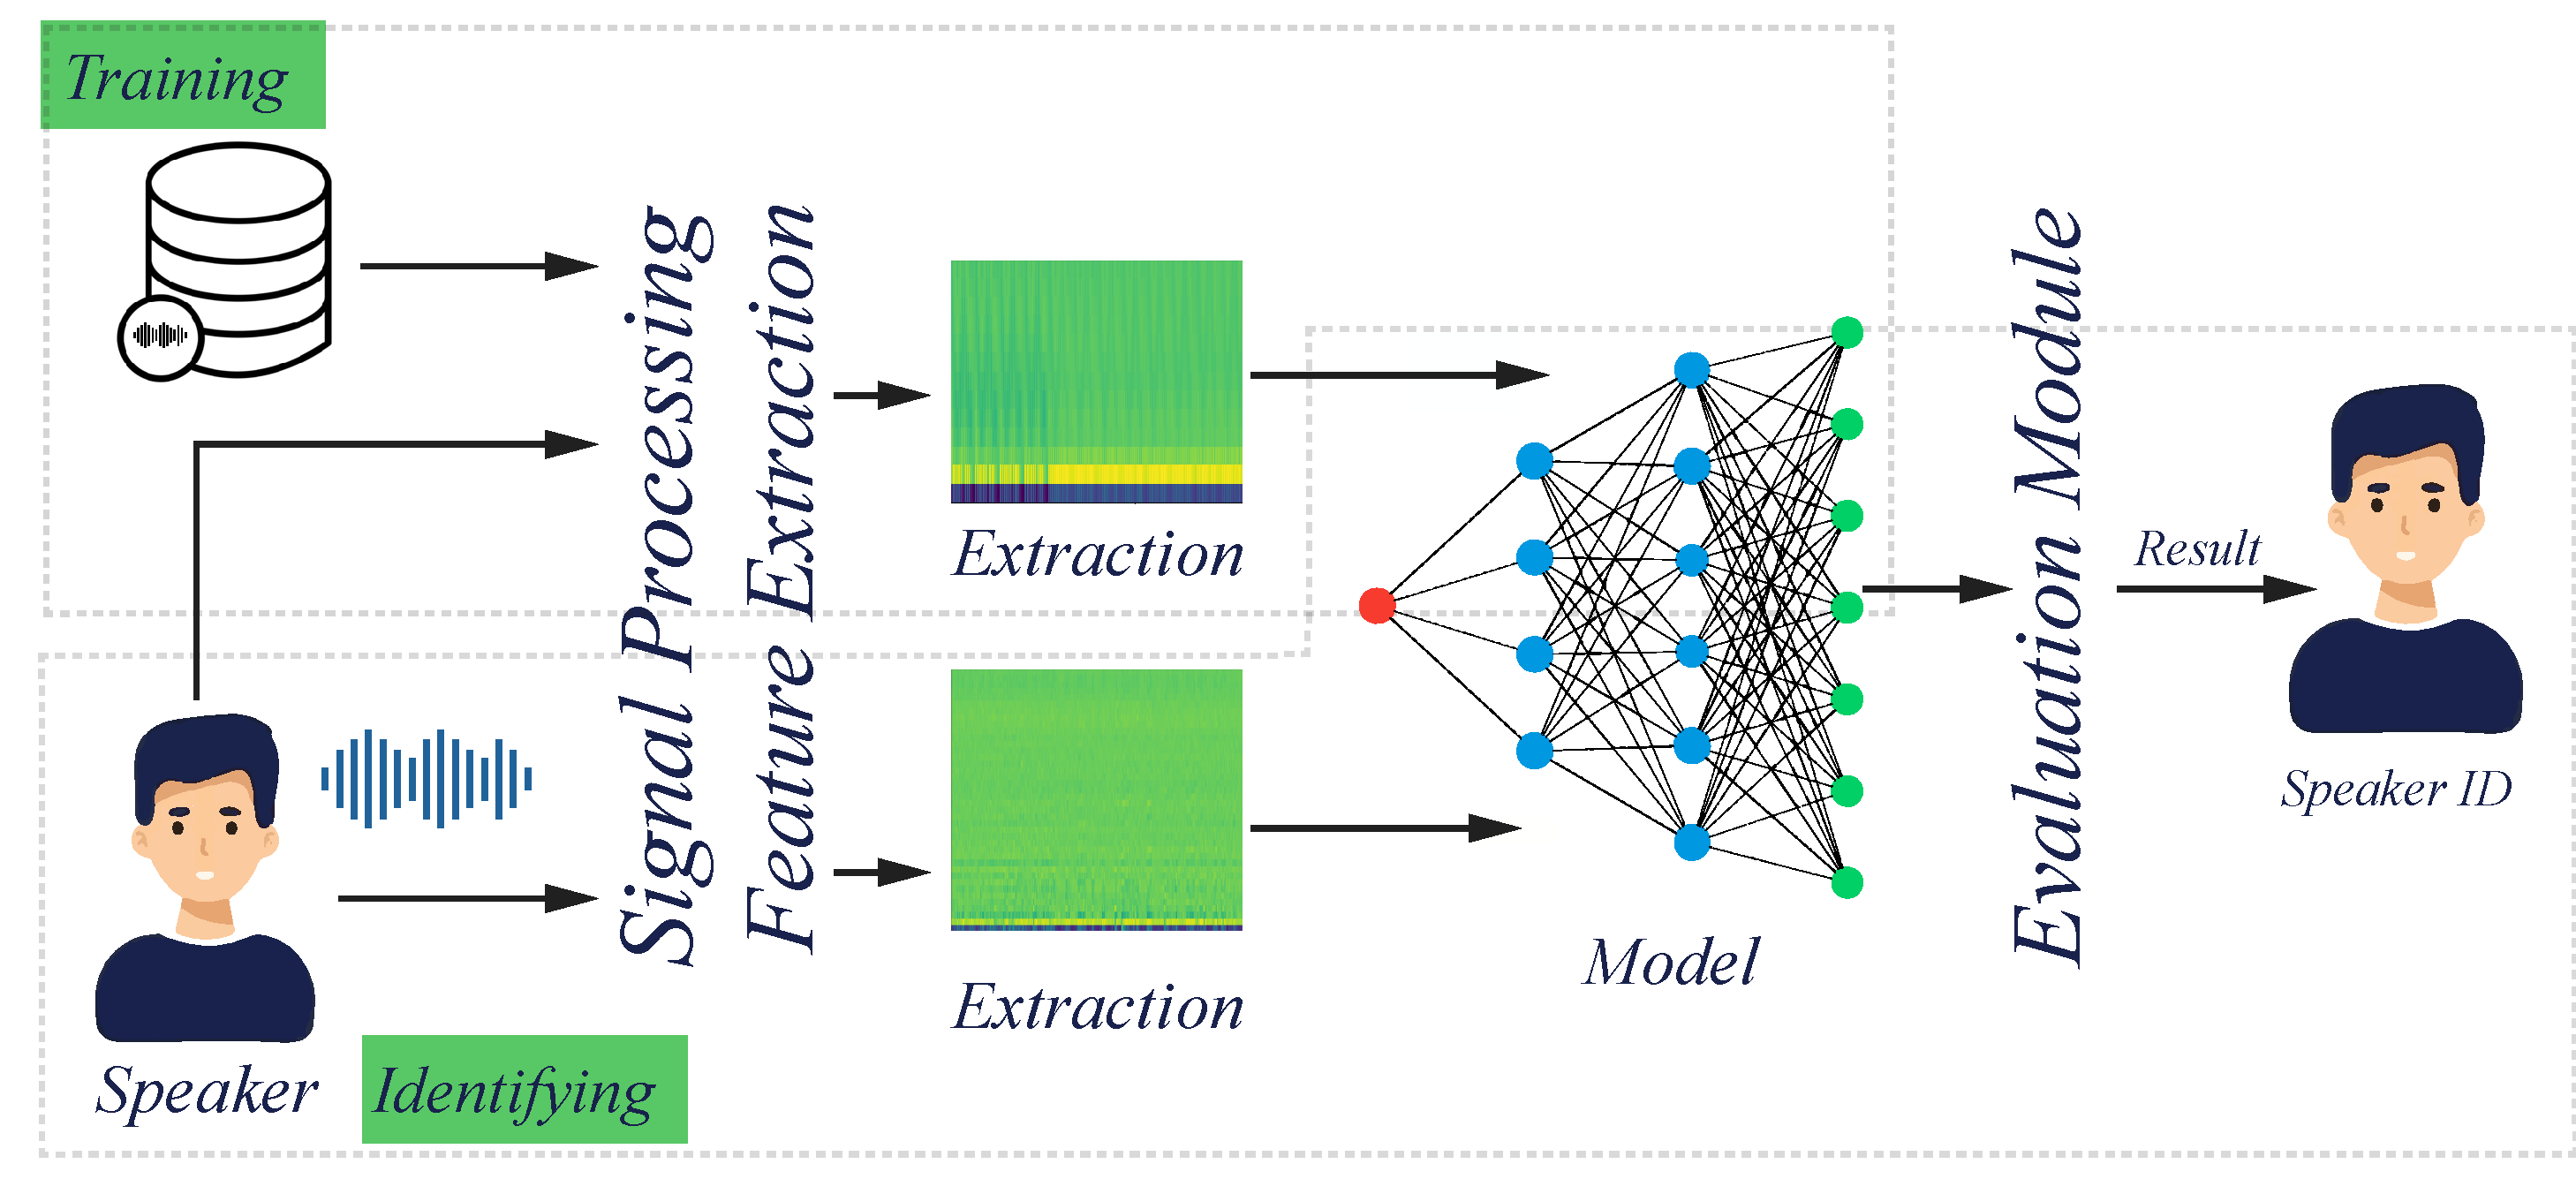
\includegraphics[width=1\textwidth]{resource/img/identification_flow.pdf}
        \caption{Speaker Identification Flow}
        \label{fig:identification_flow}
    \end{minipage}

\end{figure}


An Automatic Speech Recognition (ASR) system designed for speaker identification analyzes an input audio signal, denoted as $audio_x$.
The ASR model, represented as $f(\cdot)$, aims to match the input with the most appropriate speaker profile based on the extracted voice features.
In figure~\ref{fig:identification_flow}, when training or identifying the \textbf{feature extraction},
captures the acoustic characteristics of the input speech signal. Traditional systems often rely on \textbf{MFCC} to extract time-frequency representations of speech,
while modern systems have adopted more advanced techniques, such as \textbf{XVector}, \textbf{DVector}, and \textbf{Wavelet}, which offer enhanced representations of
speaker traits in different domains. In the next phase, \textbf{model processing}, the extracted features or raw spectrogram are fed into models such as \textbf{Hidden Markov Models (HMM)},
\textbf{Recurrent Neural Networks (RNN)}. These models map the features to an intermediate representation,
enabling accurate speaker identification. \cite{davis1980comparison, Snyder2018Xvectors,wan2018dvector,graves2013speech}.



\subsection{Hidden Markov Model (HMM)}
HMM is a probabilistic model used to describe a sequence of observations $O = \{o_1, o_2, ..., o_T\}$ through a set of hidden states $Q = \{q_1, q_2, ..., q_N\}$. In ASR

An HMM is defined by three main parameters:
\begin{itemize}
    \item $A = [a_{ij}]$: The state transition probability matrix, where $a_{ij} = P(q_{t+1} = j \mid q_t = i)$.
    \item $B = [b_j(o_t)]$: The observation (output) probability, where $b_j(o_t) = P(o_t \mid q_t = j)$.
    \item $\pi = [\pi_i]$: The initial state distribution, $\pi_i = P(q_1 = i)$.
\end{itemize}

In ASR, when a speech signal sequence is input, the goal is to find the optimal state sequence $Q^*$ that maximizes
the observation probability. When \(N\) models for each speaker is created, the Viterbi algorithm is
essential for finding the most likely state sequence based on the HMM \cite{ilyas2007speaker}.
To train the HMM, the Baum-Welch algorithm (a variant of Expectation-Maximization) is used to estimate the parameters.






\subsection{Recurrent Neural Networks (RNNs)}

Recurrent Neural Networks (RNNs) are widely used in ASR systems due to their ability to model temporal dependencies in sequential data. Unlike feedforward networks, RNNs maintain a hidden state that captures context from previous time steps, making them suitable for processing variable-length speech signals. Variants such as Long Short-Term Memory (LSTM) and Gated Recurrent Units (GRU) have been shown to effectively capture long-range dependencies and improve recognition performance \cite{graves2013speech}.

\subsection{Mel Frequency Cepstral Coefficients (MFCCs)}
Mel-Frequency Cepstral Coefficients (MFCC) are widely used in ASR systems to extract speech features by
mimicking human auditory perception. The analog speech signal is first digitized, then passed through a
high-pass filter and windowed to minimize noise and spectral leakage. The Discrete Fourier Transform (DFT)
converts the signal to the frequency domain, which is then mapped to the Mel scale. A logarithmic function
is applied to compress the dynamic range, and the Discrete Cosine Transform (DCT) converts this to the cepstral
domain. Finally, first- and second-order derivatives ($\Delta$, $\Delta^2$) are added to capture temporal dynamics. \cite{davis1980comparison}















\subsection{Wavelet}

In this work, we use the Discrete Wavelet Transform (DWT) to extract features
from audio signals for speaker identification. Unlike the Fourier Transform,
which only captures frequency content, the DWT provides both time and frequency information, making it suitable for analyzing non-stationary signals like speech.

Given an input signal, the DWT decomposes it into approximation and detail
coefficients at multiple levels using a pair of low-pass and high-pass filters followed by downsampling. This hierarchical decomposition allows for capturing transient and localized features in speech.

We use the Daubechies-4 (db4) wavelet and apply the transform up to level 1.
From each set of wavelet coefficients, we extract statistical features such as mean, standard deviation, max, min, median, and energy. These features serve as inputs for a Gaussian Hidden Markov Model (HMM) classifier or Recurrent Neural Network (RNN). \cite{tufekci2000dwt}















\subsection{X-Vector}

The X-Vector model uses a deep neural network to generate speaker embeddings. It consists of:

\begin{itemize} \item \textbf{Preprocessing}: Filters input features for localization.
    \item \textbf{Frame-level layers}: Convolutional or TDNN layers extract
          frame-level features. \item \textbf{Statistics pooling}: Aggregates
          features across the utterance using statistics (e.g., mean, standard deviation).
    \item \textbf{Speaker embedding}: Produces a fixed-length X-Vector
          representing speaker-specific information. \end{itemize}


In this study, we use the pre-trained X-Vector model from the SpeechBrain
library to extract speech features from audio segments. The X-Vector model
is based on a deep neural network architecture, trained on large
datasets: VoxCeleb to learn feature vector representations
for individual speakers.




\subsection{D-Vector}

The \textbf{D-Vector} is a speaker embedding method that captures speaker-specific
characteristics from short speech segments. It is typically extracted from the
bottleneck or penultimate layer of a deep neural network trained for speaker
classification. These embeddings are widely used in speaker verification,
diarization, and voice cloning tasks due to their ability to represent speaker
identity compactly and effectively.

As introduced by Variani et al.~\cite{variani2014deep}, the D-Vector system employs
a deep neural network with a softmax output layer to classify speakers, and the
output of an intermediate layer is used as the speaker embedding.


In this paper, we use the SpeechBrain's SpeakerRecognition class to load the pre-trained
ECAPA-TDNN model. This model is designed to extract high-quality speaker embeddings.
Then we used the Hidden Markov Models, Recurrent Neural Network,
Quantum Convolutional Neural Network to perform training.










\section{Combination Enhancement}

We present our proposed models for speaker identification, which incorporate a novel Quantum Convolutional Neural Network (QCNN) architecture, along with a hybrid model that combines traditional Hidden Markov Models (HMM) and QCNN. Unlike conventional methods like RNNs or HMMs that rely on standard neural network architectures, our approach leverages quantum-enhanced processing to better capture both temporal and spectral features in speech signals.

\subsection{Overview}

The overall pipeline consists of the following stages: audio preprocessing, feature extraction (MFCC, Wavelet, X-vector or D-Vector), quantum encoding, QCNN modeling, and speaker classification. For the hybrid approach, we introduce a post processing stage using Hidden Markov Models (HMMs) to capture temporal consistency in speaker transitions. Figure~\ref{fig:pipeline} illustrates the overall system architecture.
\tikzset{
block/.style = {
        rectangle, draw=black, fill=blue!10,
        rounded corners, minimum height=1.2em, minimum width=6em,
        font=\scriptsize, text centered, text width=6em
    },
line/.style = {draw, thick, -{Latex[length=2mm]}, shorten >=2pt},
optional/.style = {block, fill=orange!20},
output/.style = {block, fill=green!20}
}
\begin{figure}[ht]
    \centering
    \begin{tikzpicture}[node distance=0.9cm and 0.9cm]

        % Top to bottom
        \node[block] (audio) {Audio};
        \node[block, right=of audio] (pre) {Preprocessing};
        \node[block, right=of pre] (feat) {Feature Extraction};

        % Left to right
        \node[block, below=of feat] (encode) {Quantum Encoding};
        \node[block, below=of encode] (qcnn) {QCNN};
        \node[optional, below=of qcnn] (hmm) {HMM};
        \node[output, left=1.8cm of hmm] (out) {Speaker Prediction};

        % Edges
        \path[line] (audio) -- (pre);
        \path[line] (pre) -- (feat);
        \path[line] (feat) -- (encode);
        \path[line] (encode) -- (qcnn);
        \path[line] (qcnn) -- (out);
        \path[line] (qcnn) -- (hmm);
        \path[line] (hmm) -- (out);

    \end{tikzpicture}
    \caption{Speaker identification pipeline with quantum-classical hybrid model.}
    \label{fig:pipeline}
\end{figure}
\subsection{Feature Extraction}

We use some feature extractors such as Mel Frequency Cepstral Coefficients (MFCCs), Wavelet transform, X-Vectors, D-Vectors to extract features from raw audio segments corresponding to each speaker. In experiments with X-Vectors and D-Vectors, we use a pre-trained speaker model from SpeechBrain to capture high-level speaker characteristics.

\subsection{Quantum Encoding and Circuit Design}
This section represent the quantum feature mapping process. Our quantum circuit approach combines principles of quantum encoding with randomized parameterization. The circuit operates in two distinct phases:

\subsubsection{Initial State Preparation}
We use Hadamard gate to init each qubit in a superposition state, then apply randomly parameterized rotation:
\[
    |\psi_{\text{init}}^{(i)}\rangle = RY(\theta_i) \cdot H |0\rangle
\]
where $\theta_i \sim \mathcal{U}(-\pi, \pi)$ is sampled from a uniform distribution. This applies to all qubits $i \in \{0, 1, \ldots, n-1\}$ where $n=7$ is the total number of qubits.

\subsubsection{Entanglement Layer}
Adjacent qubits are entangled using CNOT gates, and also some additional random rotations are applied to target qubits:
\[
    |\psi_{\text{ent}}^{(i,i+1)}\rangle = RY(\phi_{i+1}) \cdot \text{CNOT}_{i,i+1} |\psi_{\text{init}}\rangle
\]
where $\phi_{i+1} \sim \mathcal{U}(-\pi, \pi)$ is also sampled from a uniform distribution. This entanglement structure is applied sequentially for $i \in \{0, 1, \ldots, n-2\}$.

The complete quantum state preparation can be expressed as:
\[
    |\psi_{\text{out}}\rangle = \prod_{i=0}^{n-2} U_{\text{ent}}^{(i,i+1)} \prod_{i=0}^{n-1} U_{\text{init}}^{(i)} |0\rangle^{\otimes n}
\]

\subsubsection{Measurement}
For classification, we measure the expectation values of Pauli-Z operators on each qubit:
\[
    \langle Z_i \rangle = \langle\psi_{\text{out}}|Z_i|\psi_{\text{out}}\rangle, \quad i \in \{0,1,2,3,4,5,6\}
\]

While the circuit accepts an input parameter, our implementation uses random parameterization rather than direct encoding of input features. This approach allows us to explore the quantum feature space through stochastic sampling, which can be advantageous for certain classification tasks.

\subsection{Quantum Convolutional Neural Network (QCNN)}

The QCNN model consists of alternating quantum convolution and pooling layers followed by a variational layer for classification. Each convolutional unit applies a fixed entangling circuit to local qubit pairs, defined as:
\[
    U^{(i,j)}_{\text{conv}} = RZ_i(\theta) \cdot CX_{ij} \cdot RZ_j(\phi) \cdot CX_{ji} \cdot RZ_i(\lambda)
\]

Pooling layers reduce the number of qubits to minimize data size, Quantum aggregation typically uses qubit measurements or control gates to discard unimportant information. A final variational block applies trainable rotations and entanglements to the reduced state, followed by measurement on selected qubits to obtain classification logits.

\subsection{Hybrid QCNN + HMM Model}

We propose a hybrid architecture that combines Quantum Convolutional Neural Networks (QCNN) with Hidden Markov Models (HMM). In this approach, we will not use QCNN as a standalone model, but we will use it to transform features extracted by standard feature extractors (e.g., MFCC, D-Vector) through a combination of quantum convolution, entanglement, and pooling operations as mentioned in Sections \textit{Quantum Encoding and Circuit Design} and \textit{Quantum Convolutional Neural Network (QCNN)}. We will then combine these transformed features with the original extracted features. The transformed QCNN features act as high-level representations, while the original features retain lower-level spectral and temporal cues. Then we will use the combined features to train the HMM for speaker identification.

Each hidden state in HMM represents a potential speaker identity, while the observation probabilities are computed using the enriched feature vectors. This combination allows the model to leverage both the discriminative power of quantum-enhanced feature transformation and the temporal consistency of HMMs, resulting in more robust speaker identification.

As mentioned in Fig \ref{fig:identification_flow}, we will add an additional step after feature extraction, processing the extracted features through QCNN and then we will combine the original features with the transformed ones to train or identify speakers. Fig \ref{fig:qcnn_flow}, show how it works.

\begin{figure}[H]
    \centering
    \begin{minipage}{0.5\textwidth}
        \centering
        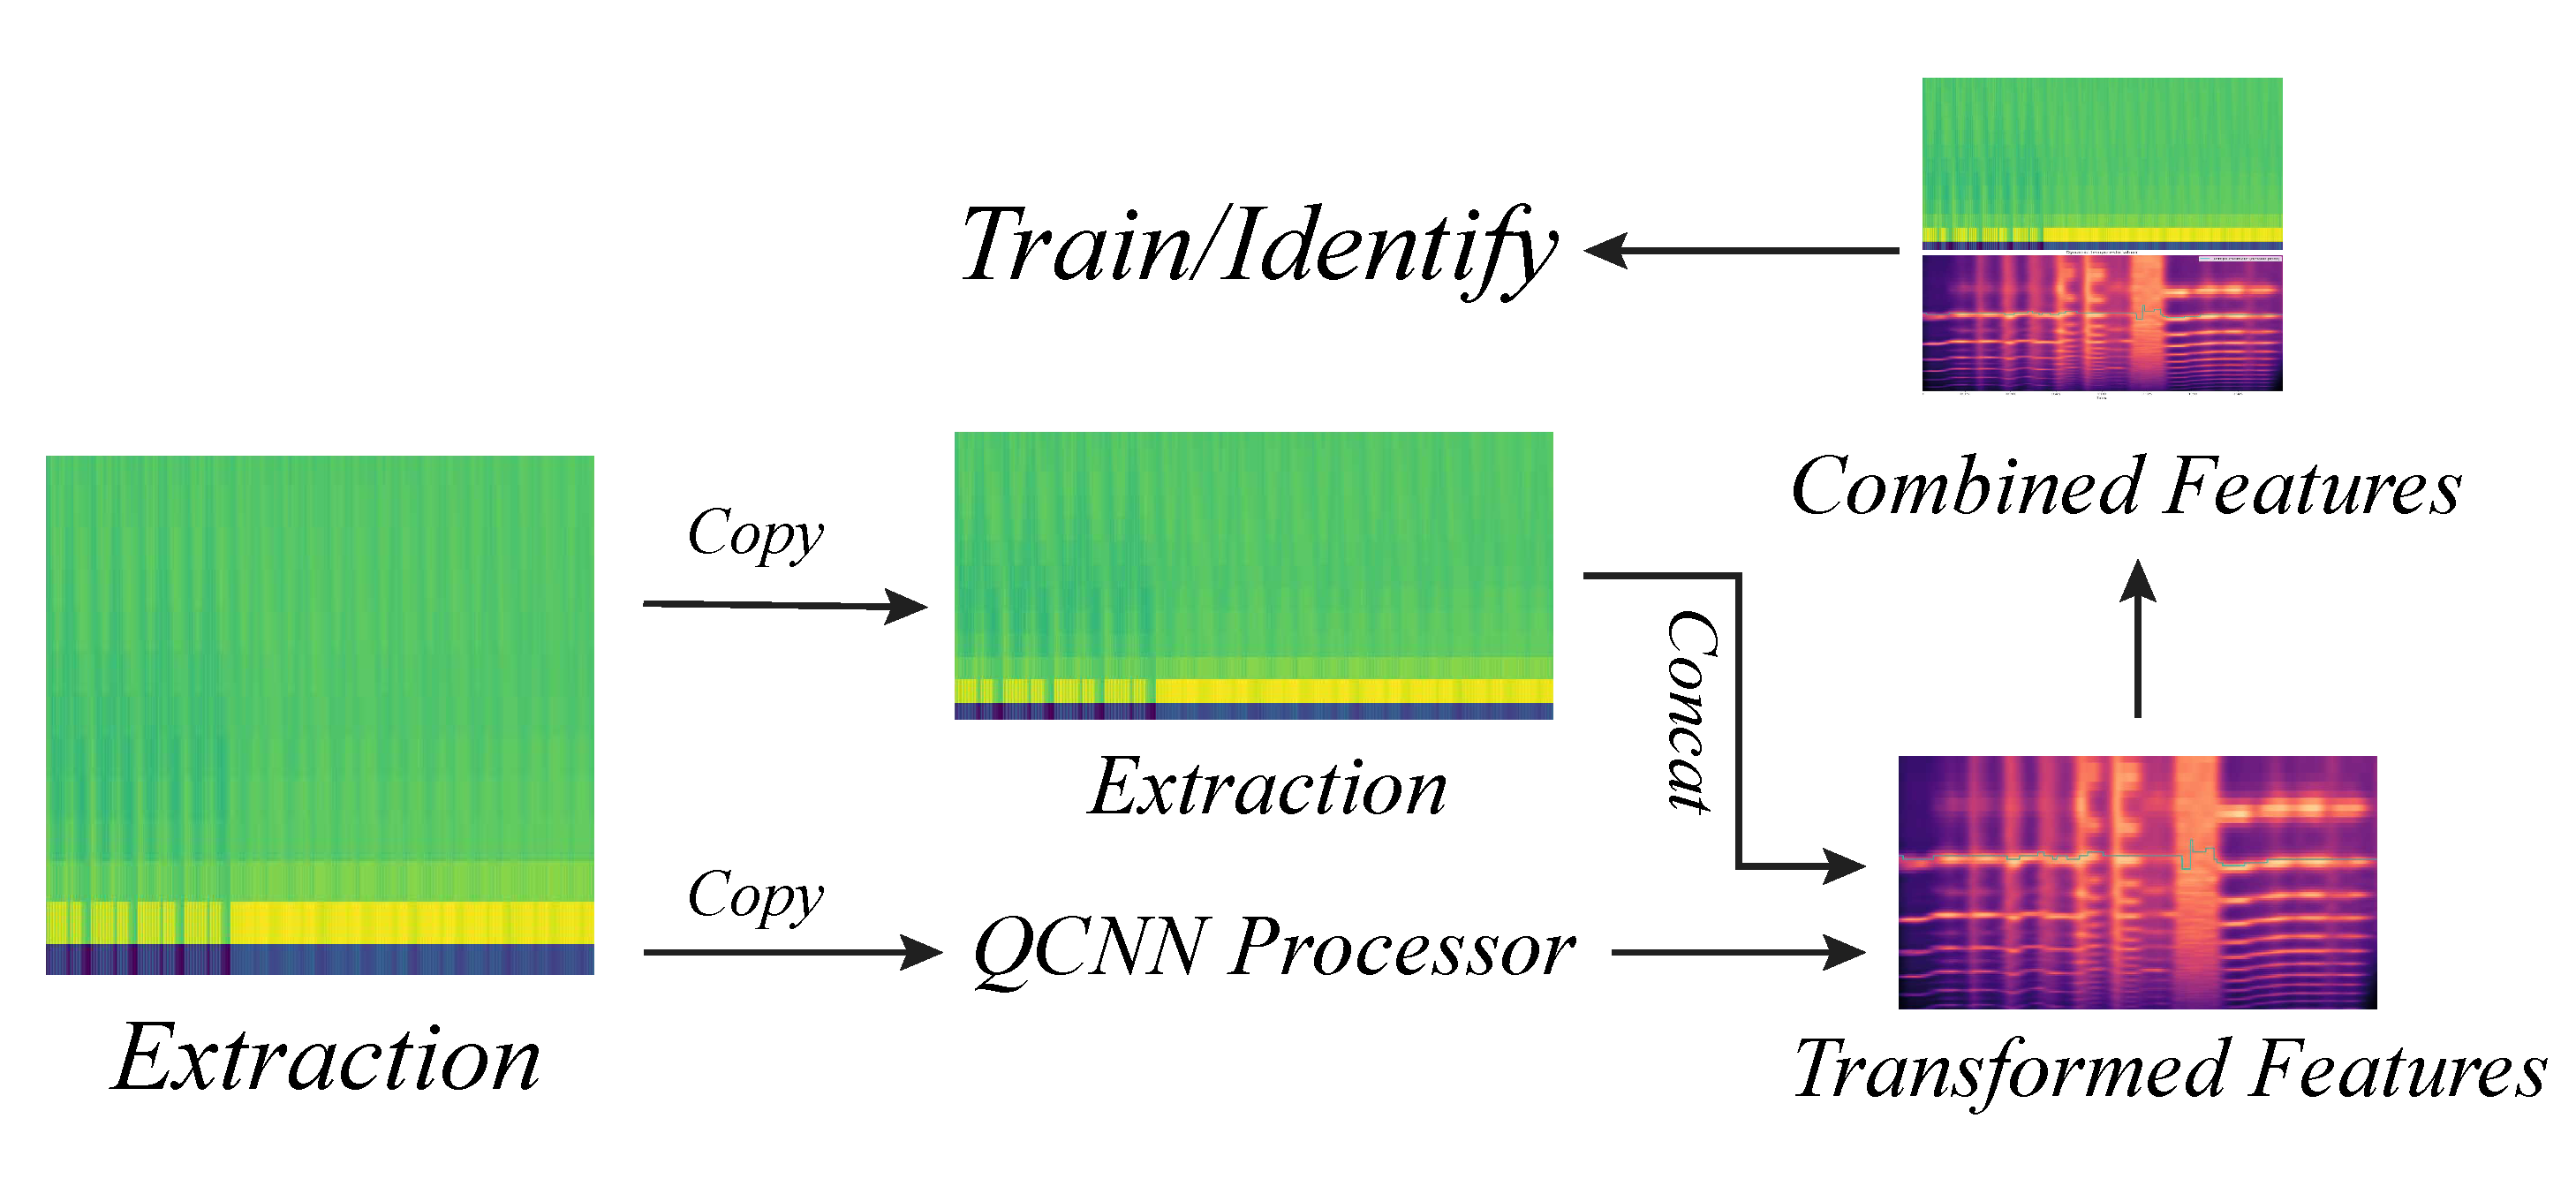
\includegraphics[width=1\textwidth]{resource/img/qcnn_flow.pdf}
        \caption{QCNN Flow}
        \label{fig:qcnn_flow}
    \end{minipage}

\end{figure}
\subsection{Training and Evaluation}

Our proposed models are trained using a cross-entropy loss on speaker labels, with parameter-shift rules applied to compute quantum gradients. For the hybrid model, once the QCNN is trained, we use the Baum-Welch algorithm to train the HMM based on the combined features (original + transformed). Evaluation is performed through cross-validation, and we report accuracy, precision, recall, and F1-score on both held-out speakers and unseen audio segments to assess generalization and robustness.


\section{Experiments}
\subsection{Experiment Setup}
We evaluated our proposed models using a curated Vietnamese speech dataset comprising various conversational contexts, including natural dialogues, group discussions, podcasts, lectures, and interviews.
The total size of the dataset is 15GB, with many measurements listed below:
\begin{table}[h]
    \centering
    \caption{Overview of speech dataset statistics}
    \begin{tabular}{|l|c|}
        \hline
        \textbf{Statistic}                  & \textbf{Value}               \\
        \hline
        Total number of speakers            & 83                           \\
        Total number of dialogues           & 10,430                       \\
        Number of speaker changes           & 751                          \\
        Total number of audio files         & 85                           \\
        Total number of script files (.txt) & 85                           \\
        Total duration of dataset           & 64,608 seconds (17.93 hours) \\
        Average dialogue length             & 6.19 seconds                 \\
        Standard deviation of length        & 11.96 seconds                \\
        \hline
    \end{tabular}
\end{table}

\subsection{Evaluation Results}
We use cross-validation to train and test many model–extractor combinations, and we obtained the results show in table \ref{tab:asr-results}.

\begin{table*}[htbp]
    \centering
    \caption{Evaluation Results of Different ASR Models Across Folds}
    \label{tab:asr-results}
    \resizebox{\textwidth}{!}{
        \begin{tabular}{|l|c|c|c|c|c|c|c|c|c|c|c|c|c|c|c|c|}
            \hline
            \textbf{Metric / Fold} & HMM-MFCC & HMM-XVec & HMM-Wavelet & HMM-DVec & RNN-MFCC & RNN-XVec & RNN-Wavelet & RNN-DVec & QCNN-MFCC & QCNN-Wavelet & QCNN-XVec & QCNN-DVec & QCNN-HMM-MFCC & QCNN-HMM-Wavelet & QCNN-HMM-XVec & \textbf{QCNN-HMM-DVec} \\
            \hline
            Accuracy Fold 1        & 0.49     & 0.66     & 0.15        & 0.36     & 0.78     & 0.69     & 0.39        & 0.86     & 0.42      & 0.16         & 0.11      & 0.44      & 0.83          & 0.32             & 0.95          & \textbf{0.97}          \\
            Accuracy Fold 2        & 0.55     & 0.71     & 0.18        & 0.36     & 0.79     & 0.70     & 0.39        & 0.86     & 0.42      & 0.21         & 0.11      & 0.49      & 0.82          & 0.33             & 0.95          & \textbf{0.97}          \\
            Accuracy Fold 3        & 0.48     & 0.67     & 0.17        & 0.35     & 0.78     & 0.75     & 0.39        & 0.86     & 0.56      & 0.18         & 0.11      & 0.48      & 0.83          & 0.34             & 0.95          & \textbf{0.97}          \\
            \hline
            Precision Fold 1       & 0.74     & 0.67     & 0.23        & 0.04     & 0.59     & 0.27     & 0.15        & 0.80     & 0.06      & 0.04         & 0.00      & 0.07      & 0.89          & 0.26             & 0.96          & \textbf{0.97}          \\
            Precision Fold 2       & 0.74     & 0.74     & 0.27        & 0.04     & 0.70     & 0.34     & 0.17        & 0.80     & 0.06      & 0.07         & 0.00      & 0.07      & 0.88          & 0.26             & 0.96          & \textbf{0.97}          \\
            Precision Fold 3       & 0.76     & 0.66     & 0.22        & 0.04     & 0.63     & 0.39     & 0.17        & 0.80     & 0.36      & 0.04         & 0.00      & 0.08      & 0.88          & 0.27             & 0.97          & \textbf{0.98}          \\
            \hline
            Recall Fold 1          & 0.69     & 0.59     & 0.12        & 0.10     & 0.53     & 0.28     & 0.14        & 0.74     & 0.09      & 0.05         & 0.01      & 0.10      & 0.87          & 0.19             & 0.93          & \textbf{0.95}          \\
            Recall Fold 2          & 0.73     & 0.62     & 0.15        & 0.10     & 0.58     & 0.32     & 0.15        & 0.73     & 0.07      & 0.06         & 0.01      & 0.13      & 0.85          & 0.19             & 0.90          & \textbf{0.92}          \\
            Recall Fold 3          & 0.71     & 0.56     & 0.12        & 0.10     & 0.56     & 0.39     & 0.16        & 0.74     & 0.31      & 0.04         & 0.01      & 0.13      & 0.86          & 0.21             & 0.92          & \textbf{0.94}          \\
            \hlineđ
            F1-score Fold 1        & 0.64     & 0.59     & 0.11        & 0.05     & 0.54     & 0.25     & 0.13        & 0.75     & 0.07      & 0.03         & 0.00      & 0.07      & 0.87          & 0.18             & 0.94          & \textbf{0.96}          \\
            F1-score Fold 2        & 0.66     & 0.63     & 0.14        & 0.05     & 0.59     & 0.30     & 0.14        & 0.74     & 0.05      & 0.04         & 0.00      & 0.08      & 0.85          & 0.17             & 0.92          & \textbf{0.94}          \\
            F1-score Fold 3        & 0.66     & 0.57     & 0.13        & 0.05     & 0.57     & 0.37     & 0.15        & 0.75     & 0.30      & 0.03         & 0.00      & 0.09      & 0.86          & 0.19             & 0.94          & \textbf{0.95}          \\
            \hline
        \end{tabular}
    }
\end{table*}
\subsection{Comparison of Models and Discussion}

Table~\ref{tab:asr-results} presents the performance of different ASR models evaluated across three cross-validation folds. From the results, it is evident that there are significant differences in performance depending on the feature extraction methods and the model architectures used.

We experimented some traditional models like HMM combined with MFCC or Wavelet features achieved moderate accuracy, but their recall and F1-score remained low, indicating limited robustness in distinguishing between speakers. We then use pre-trained XVector and DVector features with HMM, that show a slight improvement in accuracy for XVector, but DVector alone performed poorly when used with HMM without any deep learning enhancement.

RNN-based models generally outperformed the pure HMM-based approaches. The RNN + DVector model achieved a very high accuracy (up to 86\%) and consistent performance across folds, demonstrating the strength of the pretrained DVector embeddings in capturing speaker characteristics.

QCNN-based models alone (without HMM) showed inconsistent results, especially when combined with MFCC or XVector features. However, when QCNN was combined with HMM, there was a noticeable performance boost, particularly for models using DVector and XVector features. Among them, the \textbf{QCNN + HMM + DVector} model consistently achieved the highest performance across all folds, with an average accuracy of \textbf{97\%}, precision of \textbf{97\%}, recall of \textbf{94\%}, and F1-score of \textbf{95\%}.

This exceptional performance can be attributed to three key components:
\begin{itemize}
    \item \textbf{DVector embeddings} provide highly discriminative speaker features extracted using deep neural networks trained for speaker verification, capturing robust speaker characteristics even in short utterances.
    \item \textbf{Quantum Convolutional Neural Networks (QCNN)} enhance the model’s ability to learn non-linear and high-dimensional patterns from DVector features, which may not be fully captured by traditional CNNs.
    \item \textbf{Hidden Markov Models (HMM)} complement the QCNN by modeling temporal transitions in speech, which is effective in modeling and distinguishing speaker-specific vocal characteristics.
\end{itemize}

In summary, the combination of DVector embeddings, quantum-enhanced feature learning through QCNN, and temporal modeling via HMM offers a powerful and accurate architecture for speaker recognition tasks.

\section{Conclusion}

This paper presents a comparative study of multiple speaker identification models, combining a range of feature extraction methods (MFCC, Wavelet, XVector, DVector) with machine learning techniques such as HMM, RNN, and QCNN. Among all the evaluated models, the QCNN + HMM + DVector combination achieved the best overall performance, with an average accuracy of 97\% and an F1-score of 95\% across three folds (see Table~\ref{tab:asr-results}). These results highlight the strong synergy between deep speaker embeddings (DVector), quantum-inspired feature processing (QCNN), and sequential pattern modeling (HMM).

\textbf{The main contributions} of this work are as follows:
\begin{itemize}
    \item We propose a hybrid speaker identification framework that leverages DVector-based embeddings, Quantum Convolutional Neural Networks (QCNN), and Hidden Markov Models (HMM).
    \item We provide a comparative analysis against a wide range of baseline systems, highlighting the strength of quantum-enhanced architectures.
    \item A custom dataset was constructed, and rigorous k-fold cross-validation was applied to ensure robust and fair evaluation.
\end{itemize}

\textbf{The limitations} of this work include:
\begin{itemize}
    \item The quantum model training remains computationally intensive and may take a long training period.
    \item Evaluation was conducted under relatively clean and controlled audio conditions like conferences, tedtalks, podcasts, ..., without extensive testing in noisy or real-world environments.
    \item Generalization to unseen speakers from entirely different distributions was not assessed in this study.
\end{itemize}

\textbf{Future work}:
We aim to explore more diverse datasets, including multiple languages and mixed-language speech.
Our future work also focuses on improving the model's performance in noisy environments or when
the audio quality is low. On the technical side, we plan to deploy the model in real-time
applications such as voice assistants or security systems, potentially combining it with
emotion detection for more advanced and context-aware interactions

In summary, our findings demonstrate the potential of integrating quantum-inspired learning with deep speaker representations for robust and accurate speaker identification, paving the way for more advanced speech-based technologies.

\section{Acknowledgment}
This research was supported by The VNUHCM-University of Information Technology's Scientific Research Support Fund.

\bibliographystyle{IEEEtran}
\bibliography{resource/references.bib}
\end{document}
